% Please use the skeleton file you have received in the
% invitation-to-submit email, where your data are already
% filled in. Otherwise please make sure you insert your
% data according to the instructions in PoSauthmanual.pdf
\documentclass{PoS}

\title{Concept Study for the Beamforming Elevated Array for Cosmic Neutrinos (BEACON)}

\ShortTitle{BEACON}

\author{\speaker{Stephanie Wissel}\thanks{A footnote may follow.}\\
        California Polytechnic State University\\
        E-mail: \email{swissel@calpoly.edu}}

%\author{Another Author\\
%        Affiliation\\
%        E-mail: \email{...}}

\abstract{Tau neutrinos are expected to comprise one third of both the astrophysical and cosmogenic neutrino flux, but currently the flavor ratio is poorly constrained and the expected flux at energies >100 PeV is low. We present a new concept for a radio detector called BEACON sensitive to tau neutrinos with energies greater than 100 PeV in which a radio interferometer searches for upgoing tau neutrinos from a high elevation mountain. Signals from several antennas are coherently summed at the trigger level, permitting not only directional masking of anthropogenic backgrounds, but also a lower trigger threshold. Simulation studies indicate that a modest array size and small number of stations can achieve competitive sensitivity, provided the receivers are at high enough elevation. As a proof of concept, an array of four 30-80 MHz dual polarized antennas was deployed at the White Mountain Research Station.}

\FullConference{36th International Cosmic Ray Conference -ICRC2019-\\
		July 24th - August 1st, 2019\\
		Madison, WI, U.S.A.}

\begin{document}
%For oral and poster contributions, the maximum length of a paper is 8 pages including a title page and references.
\section{Motivation}
%\begin{enumerate}
%    \item 100 PeV extrapolated IceCube and GZK models predict comparable fluxes
 %   \item Different sources (unresolved IceCube sources vs. diffuse cosmic rays) predict transition in flavor ratios (right? check) as a function of energy
%    \item Neutrino landscape in the 2020s:
 %       \begin{enumerate}
  %          \item IceCube, RNO, ANITA : sensitive to different regimes of the all-flavor neutrino flux
 %           \item Missing: ability to determine the tau fraction of the all-neutrino flux 
 %           \item Flavor ratios: source structure, p$\gamma$, pp interactions, composition (paper by Learned on different flavor ratios)
  %      \end{enumerate}
   % \item BEACON : tau neutrino flux in the 100 PeV to 100 EeV regime
%A low cost, fast option that can be deployed at multiple sites
 %   \begin{enumerate}
   %     \item Scalable
     %   \item Full-sky
     %   \item Logistically simple
    %    \item Mutli-messenger science drives need for 100\% duty cycle and full sky
     %   \item Follow-up on ANITA anomalous events
   % \end{enumerate}
%x\end{enumerate}
%The discovery of a diffuse flux of astrophysical neutrinos in the energy range from 10 TeV to several PeV by IceCube expanded the reach of multi-messenger astrophysics to include neutrinos.  Cosmogenic neutrinos produced by the highest energy cosmic rays during propagation can point to the origin of the highest energy accelerators. 

Measuring the neutrino flux above 100 PeV is critical to uncovering the origin of the diffuse fluxes of both the highest energy cosmic rays and the highest energy neutrinos, and neutrino production mechanisms at the sources. The tau neutrino flux in particular can confirm the standard oscillation scenario that predicts that the muon and electron neutrinos produced at the neutrino sources oscillate into tau neutrinos in a new energy regime as well as probe other more exotic scenarios~\cite{Astro2020_fundamental}. 

The astrophysical diffuse flux of neutrinos observed by IceCube may extend to higher energies. The spectral index measured with the muon neutrino tracks suggests a hard spectrum of $E^{2.13\pm0.13}$~\cite{IceCube_muon}, while the spectral indices measured with the cascade events are softer, but extend to lower energies~\cite{HESE, combined}. It is possible that the diffuse neutrino landscape is a complex combination of multiple unresolved sources that can be better understood by extending the spectrum to higher energies. At 100 PeV, the expected flux from cosmogenic models and extensions to the IceCube flux overlap, making this region in particular a compelling energy range. 

To expand the reach of neutrino experiments into the 100 PeV to EeV energy regime requires an improvement in exposure at reasonable cost. We focus here on a concept that aims to maximize single station exposure to upgoing tau neutrinos using a phased interferometer on a high-elevation mountain. Such a concept is scalable in that multiple sites around the world can be used to achieve full sky coverage, which is particularly important for multi-messenger observations of transient bursts of neutrinos.

\section{Concept}
%Lay out baseline concept : 120deg FOV, 3 km, acceptance from taus at horizon and nearby mountains
Several existing and proposed experiments search for the radio emission from upgoing tau lepton decays resulting from tau neutrino interactions in the Earth~\cite{Auger, GRAND, Trinity, POEMMA}. The BEACON concept differs in placing a phased interferometer on a high-elevation mountain, as shown in Fig.~\ref{fig:concept}. Mountain ridges of high prominence ($>2$~km), the difference between the elevation of the peaks and the viewable valley, maximize the individual station acceptance, while still being close enough to the air showers to maintain a low energy threshold. By phasing multiple antennas together in an interferometer, sub-degree scale pointing can be achieved and background events can be localized and excluded from the trigger.

\begin{figure}[htbp]
\begin{center}
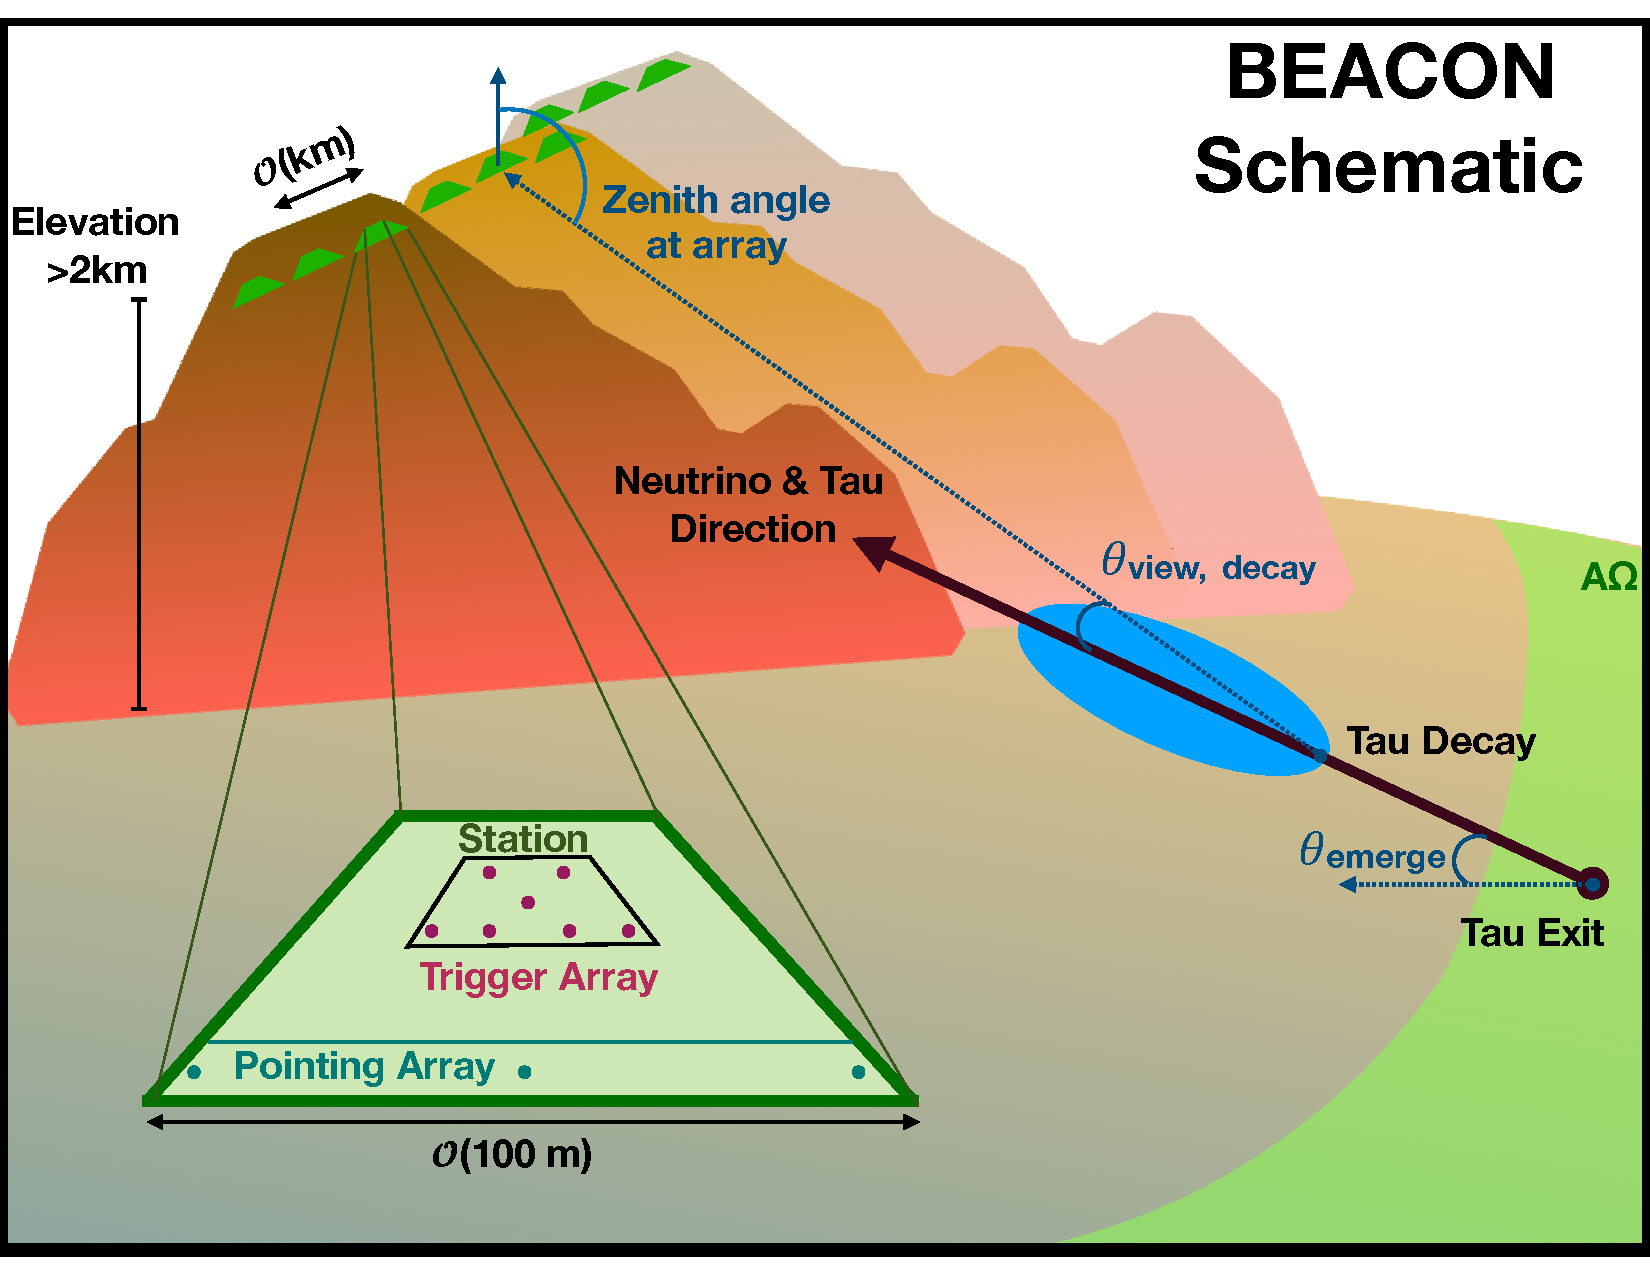
\includegraphics[width=\textwidth]{figures/BEACON_ICRC_Concept.pdf}
\caption{Concept of a high-elevation mountaintop detector.}
\label{fig:concept}
\end{center}
\end{figure}

\subsection{High Elevation Tau Detector Concept}

Upgoing tau neutrinos may be detected via the air showers that result from tau propagation and regeneration through the Earth. Tau neutrinos are expected to interact in the Earth via charged current interactions that produce a tau lepton.% which decays with a decay length of $L_{decay} = XXX$ (function that depends on density in the rock) and with energy losses governed by the inelasticity and ... 
The tau lepton decay invariably results in another tau neutrino and this process can repeat until the particles reach the other side of the Earth. When this process results in a $\tau$ lepton exiting the Earth, the $\tau$ will decay within a decay length of $L_{decay} = 49 km (E_\tau/EeV)$ to produce an air shower. The probability that a tau will exit the Earth, $P_{exit}$ depends on energy and emergence angle and is maximized for Earth skimming configurations with emergence angles $<3^{\circ}$ at energies greater than 0.1 EeV.  Tau leptons can decay through hadronic channels that produce pions or leptonic channels that produce muons or electrons. Only the hadronic and electronic decays produce air showers. We simulated the energy deposition into showers using Pythia simulated tau lepton decays, which is on average 56\% with a 68\% confidence interval of 31\%. 

Radio techniques are a promising method for the detection of ultra-high-energy particle air showers. The primary advantages are the low cost per channel of the instrumentation and the ability to trigger on showers from hundreds of kilometers away. Both are particularly important when considering the low expected flux of tau neutrinos at energies higher than 100 PeV and the geometric considerations associated with triggering on Earth skimming showers. Air showers produce broadband, impulsive signals at radio frequencies due to a combination of the geomagnetic and Askaryan effects. Cosmic rays experiments have successfully triggered on cosmic rays with radio-only triggers~\cite{TREND, OVRO-LWA} and reconstructed the air shower energies to within 14\%~\cite{AERA}.

\begin{figure}[htbp]
\begin{center}
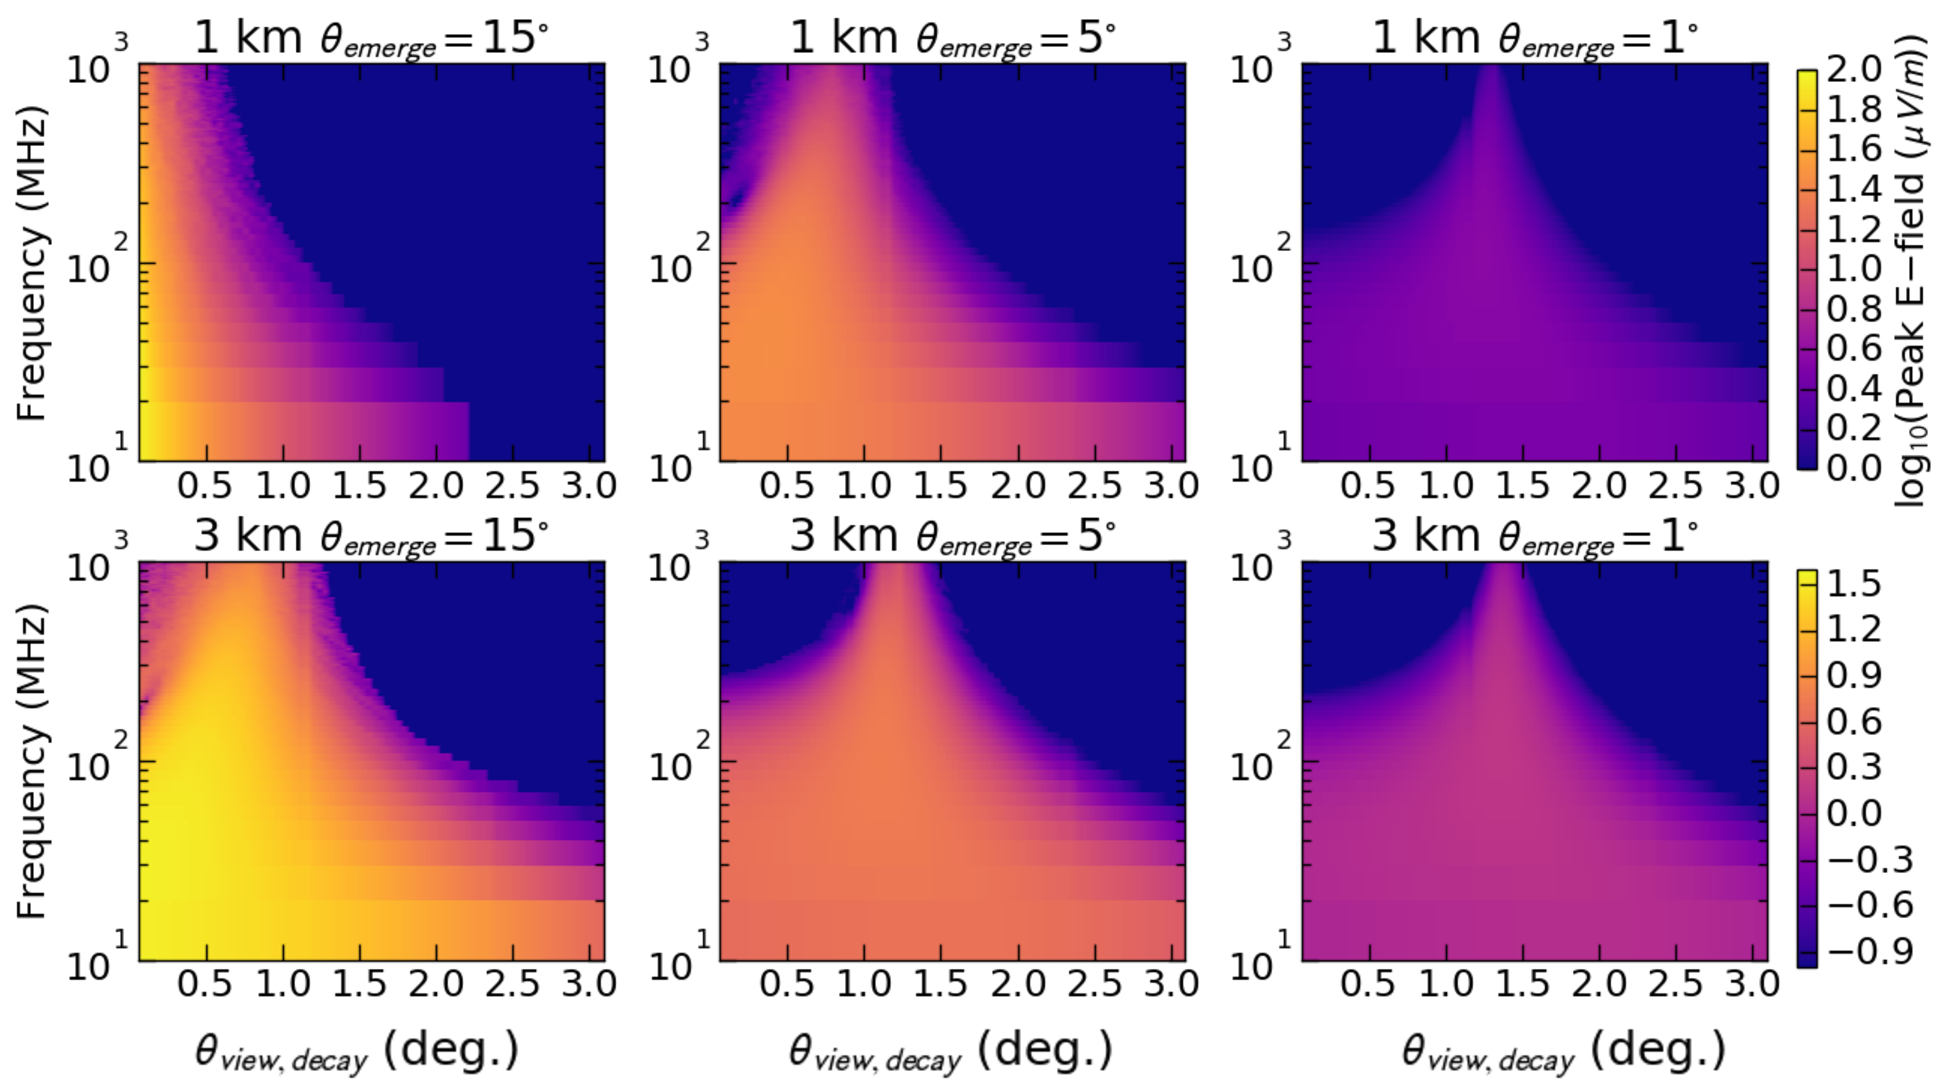
\includegraphics[width=\textwidth]{figures/efield_sims_mountainonly_logscale}
\caption{Peak electric field binned in 10~MHz subbands from ZHAireS simulations of upgoing tau lepton air showers emerging from the earth at an angle of 15$^{\circ}$ (left), 5$^{\circ}$, and 1$^{\circ}$ above the horizontal. The electric field is measured on detectors that view the shower at angles measured from tau decay point and that are placed at 1 km (top) and 3 km (bottom) elevations. }
\label{fig:efield}
\end{center}
\end{figure}

Upgoing tau air showers are expected to generate broadband electric field signals such as those shown in Fig.~\ref{fig:efield}. Using ZHAireS modified for upgoing showers, we simulated showers measured at different elevations above sea level as measured by a line of antennas. The complete set of simulations included a range of tau emergence angles from 1$^{\circ}$ to 35$^{\circ}$, view angles $\theta_{view,decay}$ relative to the decay point of the shower (0-3.2$^{\circ}$), and tau lepton decay altitudes. ZHAireS simulates the electric field in the time domain, The magnitude of the peak electric field is binned in 10~MHz subbands to form the lookup tables shown in  Fig.~\ref{fig:efield}. The radio beam is broad at lower frequencies and forms a Cherenkov cone at higher frequencies. The Cherenkov cone notably does not form when the shower is too close to the detector at, for instance, high emergence angles and low detector altitudes. 

%\begin{figure}[htbp]
%\begin{center}
%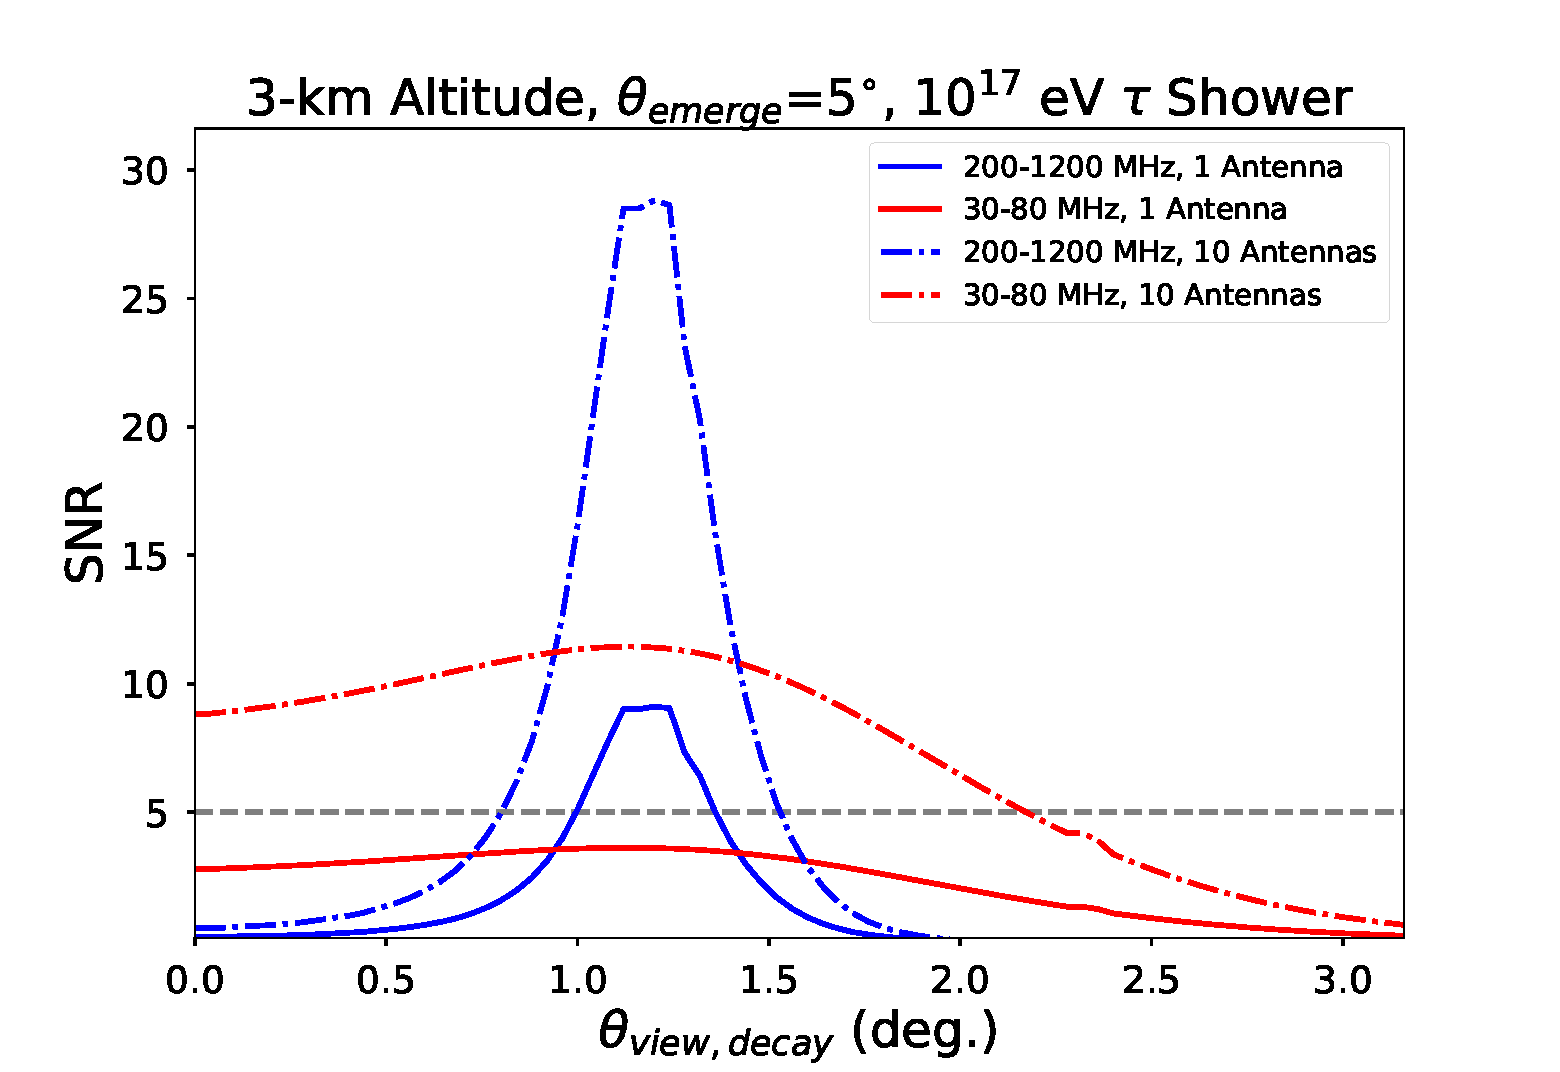
\includegraphics[width=\textwidth]{figures/SNR_example_emerge5deg_10antenna}
%\caption{Signal-to-noise ratio}
%\label{fig:SNR}
%\end{center}
%\end{figure}

An important advantage of the high-elevation radio detector design is that the detectors can be placed a multiple sites throughout the world, specifically on any mountain ridge that overlooks a reasonably radio-quiet valley. Different sites view different regions of the sky and detectors placed at mid-latitudes will in general achieve a broader sky coverage than those in the polar regions. A global network of high-elevation mountain receivers could achieve full sky coverage, an important requirement for studies of explosive transients expected from supernova, gamma ray bursts, blazar flares and others~\cite{astro_decadal}.

\subsection{Time Domain Interferometry} 

Digital interferometric triggering in the time-domain has been shown to lower the voltage field threshold of an in-ice radio neutrino experiment~\cite{oberla_ara_pa} and to self-trigger on cosmic ray air showers using an array of 500 antennas~\cite{ryan_monroe}. When used in the context of BEACON, can take advantage of several features of phased array triggering to reduce anthropogenic backgrounds at the trigger level and lower the voltage and therefore energy threshold of the detector.

Consider an impulsive, band-limited, plane wave pulse arriving at a linear phased array at an angle $\theta$ with respect to the direction perpendicular to the array. The time delay $c \delta t$ between of the signal measured at an antenna at the center of the array measured at an antenna a distance $d$ from the center of the array is given by $c \delta t = d \sin \theta$. Beams in a particular direction can be formed knowing the precise geometry of the array by delaying and summing waveforms from multiple antennas in the time-domain. Digital phased arrays form beams on an FPGA via coherent sums of $N$ antennas at programmable angles. The signal-to-noise ratio of a neutrino radio pulse grows as a factor of $\sqrt{N}$, because the signal increases by a factor of $N$ while the incoherent thermal noise grows as $\sqrt{N}$. Since the electric field emitted by a given by fully formed air shower scales linearly with the energy, increasing the SNR of weaker signals lowers the energy threshold of the detector. 

Interferometric triggering also reduces the trigger threshold of a radio array by masking out directions with strong sources of anthropogenic backgrounds. This effect was first demonstrated with the TREND experiment~\cite{TREND} and we confirm their results using both a single baseline interferometer used to survey multiple sites and a four antenna interferometer at the White Mountain Research Station. With modest baselines, we we able to reduce the noise-riding trigger thresholds from 20~$\sigma$ above the unresolved thermal noise to between 6-10~$\sigma$ over a 60$^{\circ}$ field of view. These results can be improved with improved antenna beam patterns and longer baselines, both of which are planned for the 2020 season at WMRS. Further details on the site survey and longer term instrumentation study are discussed in these proceedings~\cite{ICRC_BEACON_prototype}. 

The arrival direction of the tau neutrinos can be reconstructed using interferometric techniques as well. The one-sided beamwidth, $\Theta$, of an interferometer constructed from two antennas decreases with increasing bandwidth, $\Delta f$, and separation distance between two antennas, $L$. Coherently summing signals from $N$ antennas each with a signal-to-noise ratio at the antenna $SNR_{a}$ further narrows the interferometer's beamwidth by a factor of $SNR_{a} \sqrt{N} $. However, the SNR in the beam, $SNR_b$ also increases by $\sqrt{N}$. Combining these factors together, the pointing resolution is given by $\delta\theta \sim c/(L \Delta f SNR_b)$, meaning that a 10 antenna phased array with a bandwidth of 50 MHz and maximum baseline of 70~m can achieve a pointing resolution of $\sim0.5^{\circ}$ on a 5$\sigma$ pulse in the beam. A complete estimate of pointing resolution depends on the layout of the array and will, in general, weight the contributions from different baselines. 

%\begin{enumerate}
%    \item Interferometer 
%    \item Directional rejection of background sources
%    \item Man-made backgrounds are localized
%    \item Coherent increase in SNR
%    \item Pointing resolution limited by baseline length and radio beam width
%    \item Large single station tau neutrino exposure
%    \item High duty cycle
%    \item Large FOV per station
%    \item Sky Coverage
%    \item Mid-latitude sites permit large sky coverage
%    \item Multiple mountains to achieve full sky
%    \item Tau neutrino flux
%\end{enumerate}

\section{BEACON Detector Design Studies}\label{sec:receiver} 

%\subsection{10 Station Results}
%\begin{enumerate}
%    \item 10 antennas 
%    \item Good angular resolution
%    \item Improved sensitivity that traces the gain
%    \item Beyond this, since stations independent, better to build more stations
%    \item Differential acceptance  requires elevated antennas
%    \item Point source sensitivity
%    \item 10 station result
%    \item Acceptance
%    \item Minimum exposure required to do science
%    \item Expected event rates
%    \item Constraints on Kotera models, IceCube flux
%\end{enumerate}

%\subsection{100 Station Results}

By integrating the radio signal over different frequency ranges, we can compare the performance of a high-elevation detector in different frequency bands. We consider two bands in this study: a lower frequency band (30-80 MHz) composed of dipoles with gains of 1.8~dBi and a higher frequency band (200-1200 MHz) composed of horn antennas with gains of 10~dBi. The peak voltage in the time domain $V_{peak}$ from a tau lepton decay received on an antenna with gain $G_i$ in a frequency range $(f_{lo}, f_{high})$ is $V_{peak}=\int_{f_{lo}}^{f_{high}} E_{peak}(f)  N\frac{c}{f} \sqrt{\frac{50 \Omega }{377 \Omega} \frac{G_i(f)}{4 \pi} } df $.

The signal in both frequency bands is referenced to incoherent thermal noise which is a combination of the system temperature of the amplifier chain used in the detector,$T_{sys} = 140$~K and the antenna temperature, itself a combination of the galactic noise temperature, $T_{gal}(f)$, and the ground thermal temperature, $T_{ground}=290$~K that depends on the ratio, $r$, of the sky viewed by the antenna (assumed to be 0.5). Because galactic noise temperature follows a power law in frequency, the noise temperature assumed in these simulations is dominated by the sky noise for the lower frequency band and by the ground noise temperature in the higher frequency band. Phasing the antennas sums the noise voltage so that $V_{rms} = \int_{f_{lo}}^{f_{high}} \sqrt{N k (r T_{gal}(f)  +(1-r) T_{ground} + T_{sys}) 50 \Omega } df$, which is 14$\mu V$ for the 30-80~MHz band and 10$\mu V$ for the 200-1200~MHz band.

\begin{figure}[hbtp]
\begin{center}
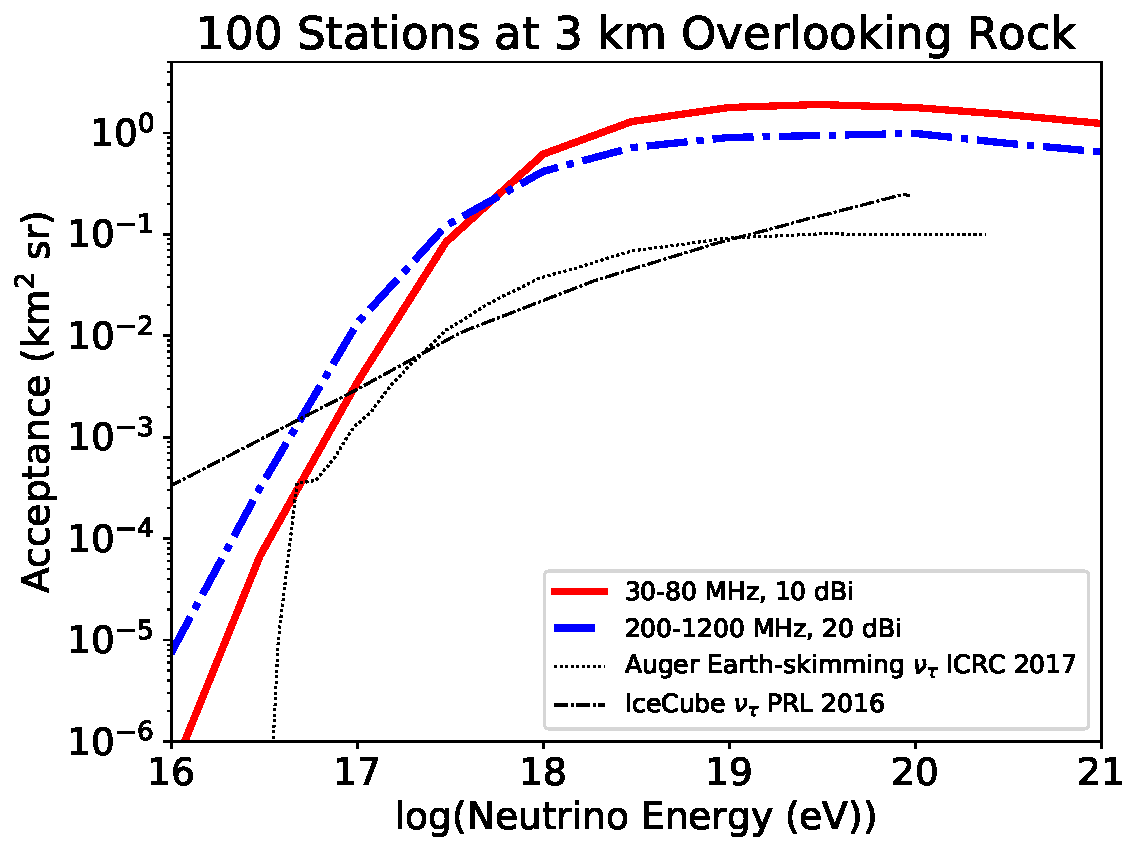
\includegraphics[width=0.54\textwidth]{figures/acceptance_100stations_energyssampling}
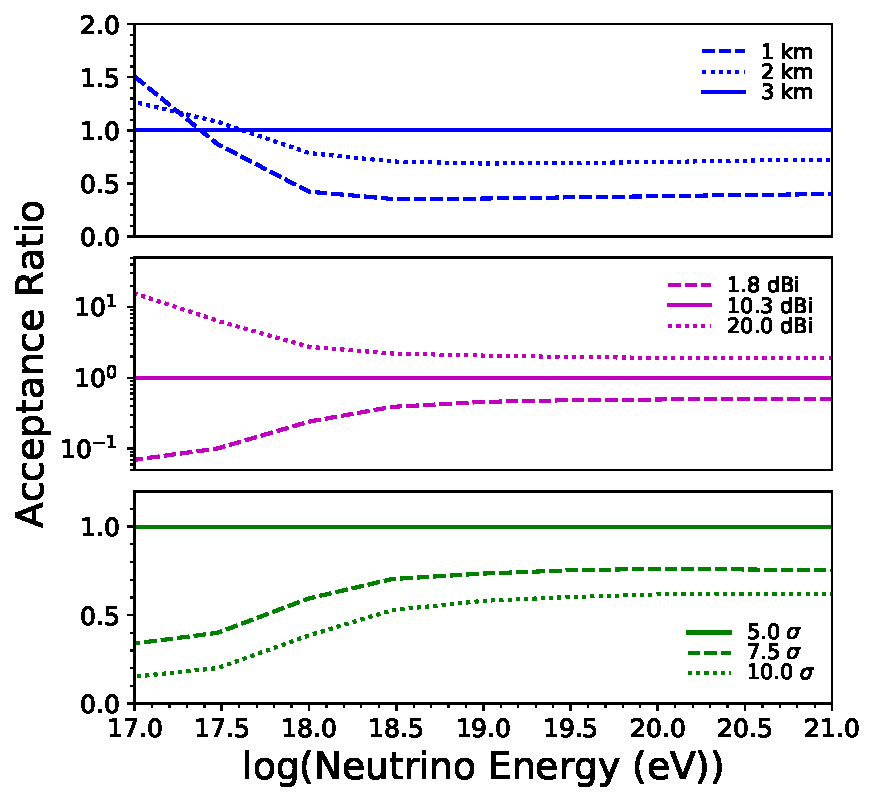
\includegraphics[width=0.45\textwidth]{figures/acceptanceratio_100stations_energyssampling_study}
\caption{(left) The acceptance of BEACON in two different frequency bands compared with the acceptance of PAO to Earth-skimming tau neutrinos and IceCube to tau neutrinos. The designs assume 100 stations at an elevation of 3 km. Each station comprises 7 antennas in the 30-80 MHz range and 10 antennas in the 200-1200 MHz range, both with a threshold of 5$\sigma$. (right) The ratio of the acceptance of a 30-80 MHz detector for different elevations (top), phased array gains (middle), and trigger thresholds (bottom) relative to the reference design. }
\label{fig:acceptance}
\end{center}
\end{figure}

The lower frequency band has a broader radio beam since the region over which the radio emission is coherent is broader at longer wavelengths. However, the peak electric field measured in the higher frequency band is stronger at the Cherenkov angle both because the bandwidth is a factor of 10 wider and also because the expected thermal noise is weaker. The 30-80 MHz band is appropriate for strong signals originating from higher energy or more distant showers, while the higher frequency band may be better for detecting closer showers or lower energy showers. This is evident in Fig.~\ref{fig:acceptance}(left) where the lower frequency band achieves a higher acceptance at energies greater than $3\times10^{17}$~eV, while the higher frequency band has a lower energy threshold.  The acceptance of a 100 stations of a high-elevation mountain detector in either frequency band improves on the acceptances of the Pierre Auger Observatory (PAO) to Earth-skimming tau neutrinos and IceCube's acceptance to tau neutrinos by a roughly a factor of 10. Given the small differences between the two frequency bands, the design frequency band will likely be better determined by the RFI local to a given site. 

The optimal design of a high elevation radio interferometer depends on several factors shown on the right in Fig.~\ref{fig:acceptance} including the detector elevation (top), the effective gain of the phased array (middle), and the average trigger threshold on the beam (bottom). The acceptance ratios are referenced to a design of a single BEACON station composed of 7 phased antennas each with a gain of 1.8 dBi and a frequency band of 30-80 MHz placed at an elevation of 3 km with a 5$\sigma$ threshold on the beam.

Detectors at higher elevation view a larger area and are far away enough from the showers that the tau lepton can decay and the air shower can fully develop. This results in a higher acceptance at energies greater than $10^{18}$~eV as the detectors are placed at higher elevation, but there is a smaller increase in the acceptance going from 1 km to 2 km than from 2 km to 3 km. For lower neutrino energies, the BEACON detector is more likely to trigger on events with a shorter distance between the shower and the detector. This suggests that mountain ridges at at least 2 km should be considered for a detector of this design, to maximize both the acceptance at the highest energies and to minimize the number of stations.

Including more antennas in a phased array increases the effective gain, $G_{eff}$ of the interferometer by $G_{eff} = 10 \log_{10} N + G_i$. While individual antennas with higher gain result in a narrower beamwidth and therefore a narrower field of view, digital phasing allows us to overlap the beams so that the full 120$^{\circ}$ field of view still contributes to the effective area. Thus increased gain lowers the energy threshold and increases the acceptance of the detector to weaker signals from higher energy showers initiated further away. However, there is only marginal benefit going from an effective gain of 10~dBI to 20~dBI; the acceptance increases by a factor of  2 at energies greater than $10^{18}$~eV while the number of required channels increases by a factor of 10. 

The trigger threshold of an impulsive radio receiver is typically implemented as a noise-riding threshold that adjusts itself through a PID loop to meet a predefined global trigger rate. Fluctuations in the local RFI environment due to anthropogenic backgrounds can cause the thresholds to vary over time and in different beams. A factor of 2 increase in the averge threshold from 5$\sigma$ to 10$\sigma$ above thermal noise in the beams results in a reduction of the acceptance of 80\% at $3\times10^{17}$~eV and 42\% at $10^{19}$~eV. We assume a trigger threshold of 5$\sigma$ for this study, based on successful implementation of the phased array technique in an ARA station~\cite{oberla_phased}.

\section{BEACON Array Design}\label{sec:array} 
\begin{figure}[tbhp]
\begin{center}
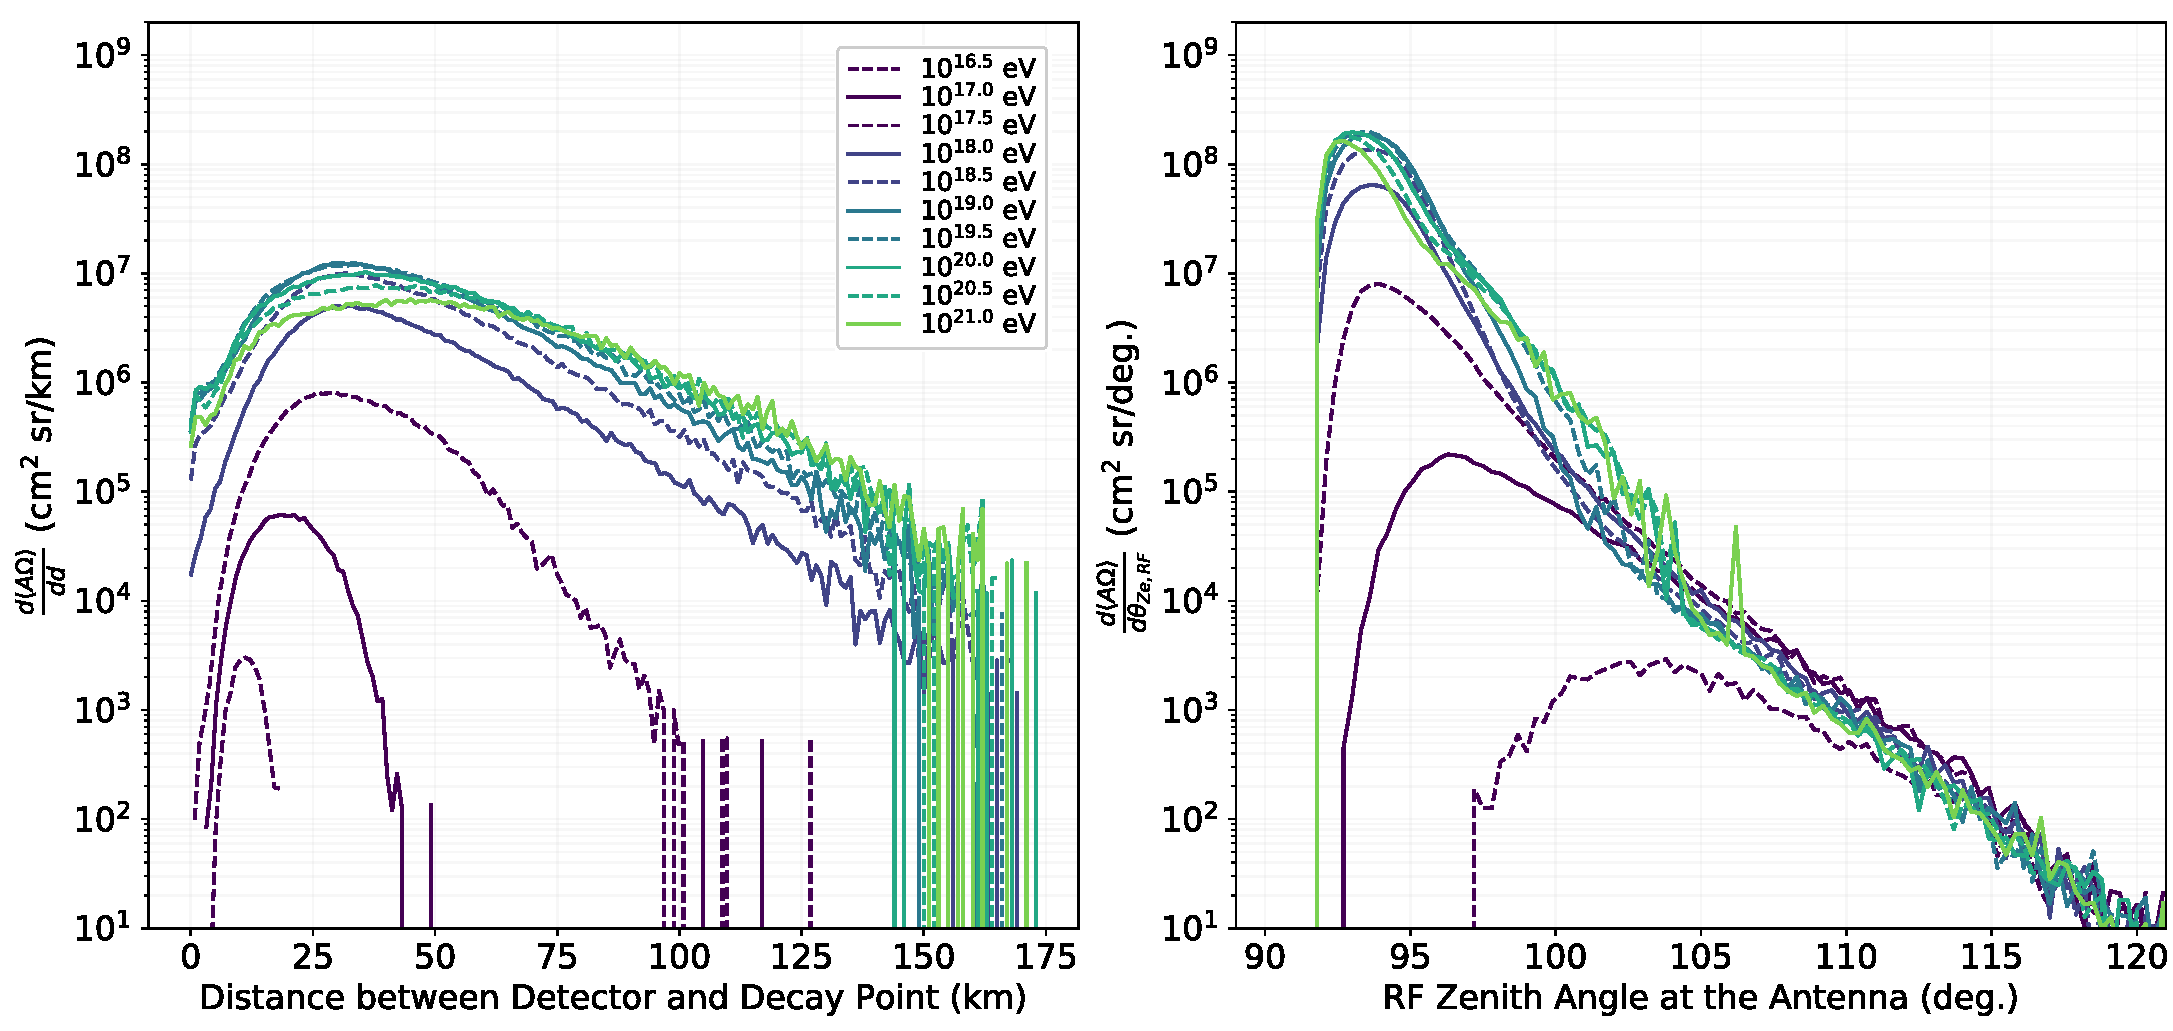
\includegraphics[width=\textwidth]{figures/diffacceptance_30-80MHz_refdesign}
\caption{Differential acceptance of the BEACON reference station to isotropoic tau neutrino flux shows the predominant distances between the decay point and the detector (left) and the zenith angles measured at the array (right) for various energies.}
\label{fig:diffaccep}
\end{center}
\end{figure}

When deciding on array layout, there is a tradeoff between the close packing desired for digital phasing and angular resolution and cosmic ray rejection. The latter two prefer longer baselines to achieve finer angular resolution, while the phasing technique presumes that the antennas are closely packed enough that each antenna in the array views a similar portion of the shower and is a similar distance from the showers. To illustrate the geometry at hand, Fig.~\ref{fig:diffaccep} shows that for high-elevation mountain geometries, triggered showers are between 10 and 100~km from the detector with lower energy showers triggering at closer distances and therefore steeper angles below the horizon. These results have two important implications. 

First, the showers are far away enough from the detectors that the signals observed over the core portion of the array are similar. A detector observing a 5$\sigma$ shower at 10~km distance and with 140~m maximum baseline separation between 10 receivers operating in the 30-80~MHz band would have a 0.3$^{\circ}$ angular resolution. Even in the conservative case that evenly spaces 10~antennas on a triangular grid, the electric field observed in a beam would be degraded by at most 3\%. 

Second, since the higher energy showers especially are expected to be concentrated into angles near the horizon, precision angular reconstruction is required for successful background rejection of the more prevalent down-going cosmic rays.  Given 10 antennas in a station, at least three of them could be used as pointing antennas placed at longer baselines, while the other 7 could be more closely packed and used primarily for triggering. 

\section{Discussion}
The results of Sections~\ref{sec:receiver} and \ref{sec:array} lead us to a reference design for a BEACON station that phases together 10 antennas in a lower frequency band (30-80~MHz) with a view of 120$^{\circ}$. The site is assumed to be at 3~km. We assume the station layout shown in Fig.~\ref{fig:concept}. This reference design is used for the results presented in Figs.~\ref{fig:acceptance}, \ref{fig:diffaccep}, and \ref{fig:number_nus}.

\begin{figure}[htbp]
\begin{center}
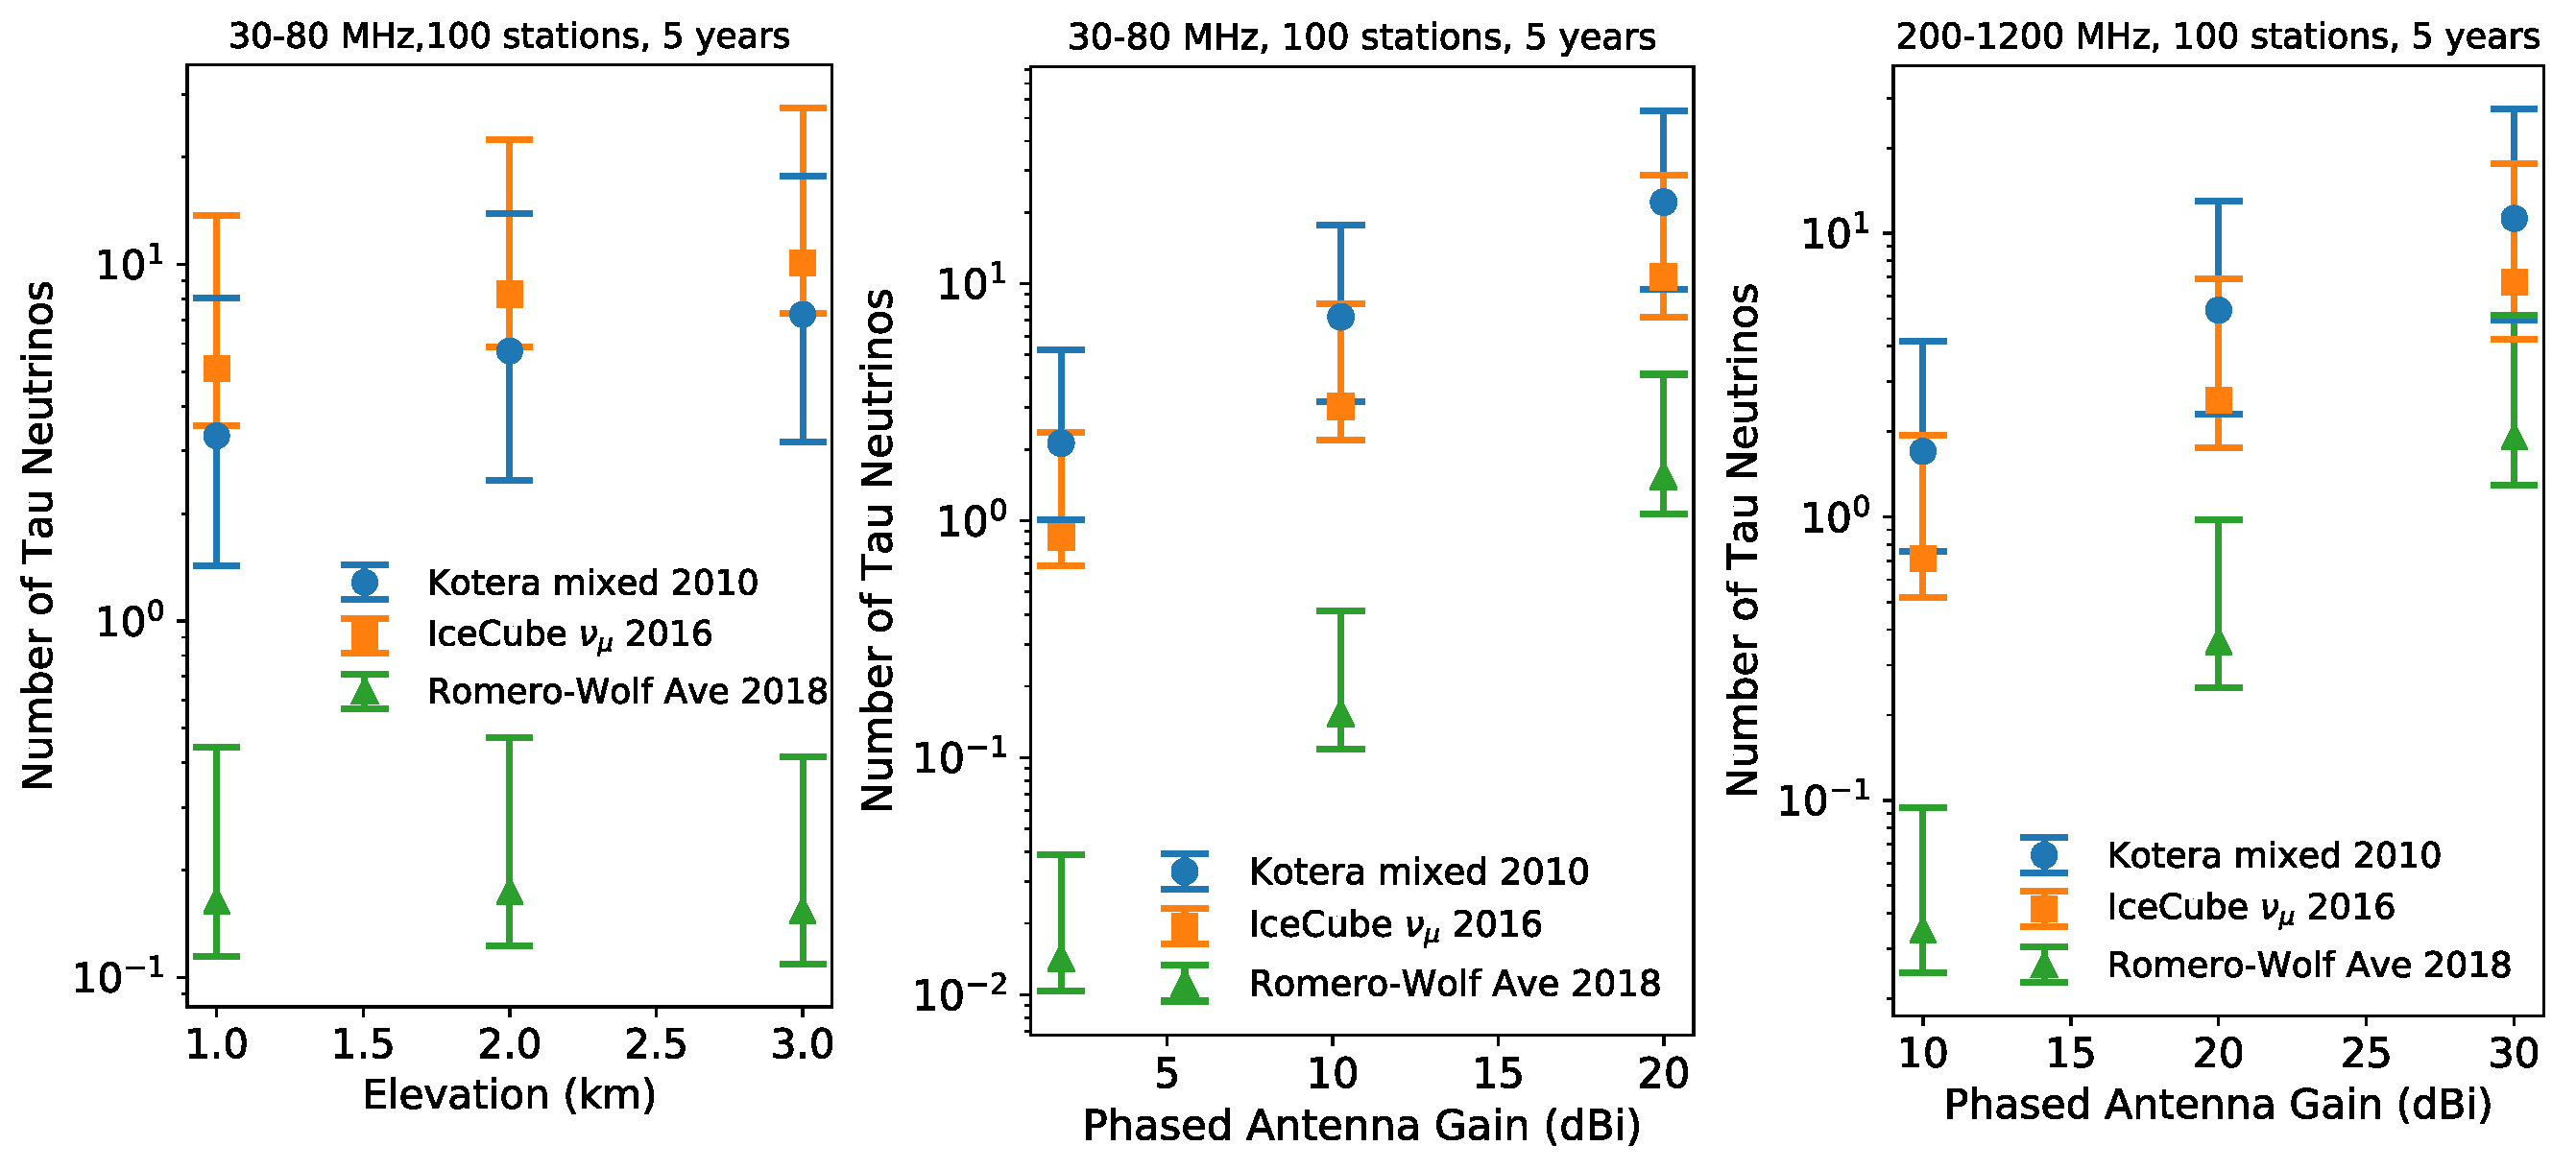
\includegraphics[width=\textwidth]{figures/beacon_5years_100stations_variations}
\caption{The number of neutrinos expected from models that have high $E_{max}$, extend the IceCube muon flux, and predict a lower $E_{max}$ with 100 stations of a BEACON detector with a 30-80 MHz design (left) at different elevations or (middle) with varying numbers of phased antennas. (right) The same as the middle figure, but with a 200-1200 MHz detector design.}
\label{fig:number_nus}
\end{center}
\end{figure}

The BEACON reference design can be compared against several types of models predicting an isotropic flux of tau neutrinos. Cosmogenic models that assume that the cutoff energy, $E_{max}$, in the accelerators is high and the harder power law measured by the IceCube muon neutrino flux predict $XX \pm XX$ and $XX \pm XX$ tau neutrinos in 5 years of observation, respectively. Other models like those that assume lower $E_{max}$ predict $XX \pm XX$ neutrinos in the same time period. Extensions to the IceCube flux based on the softer spectra made with the HESE events or cascade events predict a similar order of magnitude of neutrinos. We divide these models into two classes: those that extend to higher energy and lower energy models.

Fig.~\ref{fig:number_nus} shows the dependence of the expected number of neutrinos for three neutrino models on elevation, the frequency band, and the number of antennas included in the phased array assuming a 1:1:1 flavor ratio. The higher energy models show a factor of 2 increase in the number of neutrinos going from a 1~km elevation to a 2~km elevation, the gain going from 2~km to 3~km is marginal. The lower energy models show a weak preference for the 1 and 2~km elevations. 

Both the lower and higher energy models indicate that the increase in number of neutrinos is linear with phased gain. However, since the number of neutrinos increases linearly with the number of independent stations, we conclude that the preferred station design includes 10 antennas used for both triggering and pointing reconstruction. 

Detector concepts for the highest energy tau neutrinos based on phased arrays of radio receivers placed on high-elevation mountains take advantage of high individual station acceptance to an isotropic flux while still maintaining sub-degree pointing resolution. We are further pursuing open questions with respect to this design including the point source sensitivity to transient neutrino phenomena as well as site surveys for different possible BEACON sites and triggering on cosmic rays from a high-elevation mountain~\cite{ICRC_BEACON_prototype}.

%\section{Acknowledgements}
This work is funded in part by the National Science Foundation NSF CAREER Award \#1752922 and the Frost Fund at the California Polytechnic State University. We thank the outstanding staff at the National Science Foundation White Mountain Research Station for their support and acknowledge the use of their high-altitude facilities.

\begin{thebibliography}{99}
\bibitem{...}
....






\end{thebibliography}

\end{document}
